\vspace{-1.6em}\section{Use case 1}\label{appendix:seapp_uc1}

\vspace*{-0.5em}
In this use case we demonstrate how an app could benefit from the
fine-granularity access to files.  In particular, we show how the {\em
  UseCase1Activity}, suffering of a path traversal vulnerability,
cannot be exploited when the app is associated with a properly
configured policy module.  According to the Google Play Protect report
on common application
vulnerabilities~\cite{seapp_common_play_protect_vulnerabilites},
unsanitized path names that lead to path traversal are a primary
source of problems in applications.

{\em UseCase1Activity} is quite simple: it displays the content of a
file given its relative path through an intent
(Figure~\ref{fig:seapp_uc1_views}a). While this may be fine when the
intent comes from trusted components, the activity supports also
implicit intents coming from untrusted sources. This makes the
vulnerability easily exploitable by an attacker targeting the
confidential files written by the {\em core\_logic} components.
%
In our setup phase, we leverage {\em MainActivity} to create an
internal directory structure by using the {\tt android.os.File}
abstraction, which sets file and directory context upon its creation
(see Section~\ref{sect:seapp_impl_files}). Two directories are
created: {\tt user/} and {\tt confidential/}; inside both folders a
file {\tt data} is saved.
%
To test this use case, we first start {\em UseCase1Activity}, then we
send an intent to ``confuse'' {\em UseCase1Activity} into showing us
the content of {\tt confidential/data}. This can be done via ADB with
the command:
\begin{lstlisting}[numbers=none]
adb shell am start
-n com.example.showcaseapp/.UseCase1Activity
-a "com.example.showcaseapp.intent.action.SHOW"
--es "com.example.showcaseapp.intent.extra.PATH" "../confidential/data"
\end{lstlisting}
\normalsize

When the policy module is not availableg, all app internal files are
flagged with {\tt app\_data\_file} and every app component executes
within the {\tt untrusted\_app} domain, which holds read access to
{\tt app\_data\_file}. As a consequence the vulnerability is
successfully exploited and {\em UseCase1Activity} shows the content of
the {\tt confidential/data} file (Figure~\ref{fig:seapp_uc1_views}b).

Instead, when the policy module is available, the file {\tt
  confidential/data} is flagged with {\tt confidential\_t}, as
indicated in line 2 in \filecontexts (see
Listing~\ref{seapp_filectxp}). Since no permission is granted on {\tt
  confidential\_t} in the \sepolicy to {\tt user\_logic\_d}, any
access to the file {\tt confidential/data} by {\em UseCase1Activity}
is blocked by \sel (Figure~\ref{fig:seapp_uc1_views}c). The following
denial is written to the system log: {\em denied {\tt search} to {\tt
    user\_logic\_d} domain on {\tt confidential\_t} type}
(Figure~\ref{fig:seapp_uc1_logcat}). The {\tt confidential} directory
cannot then be accessed despite the exploitation of the path traversal
vulnerability.

\begin{figure}[h!]
  \centering
  \subfloat{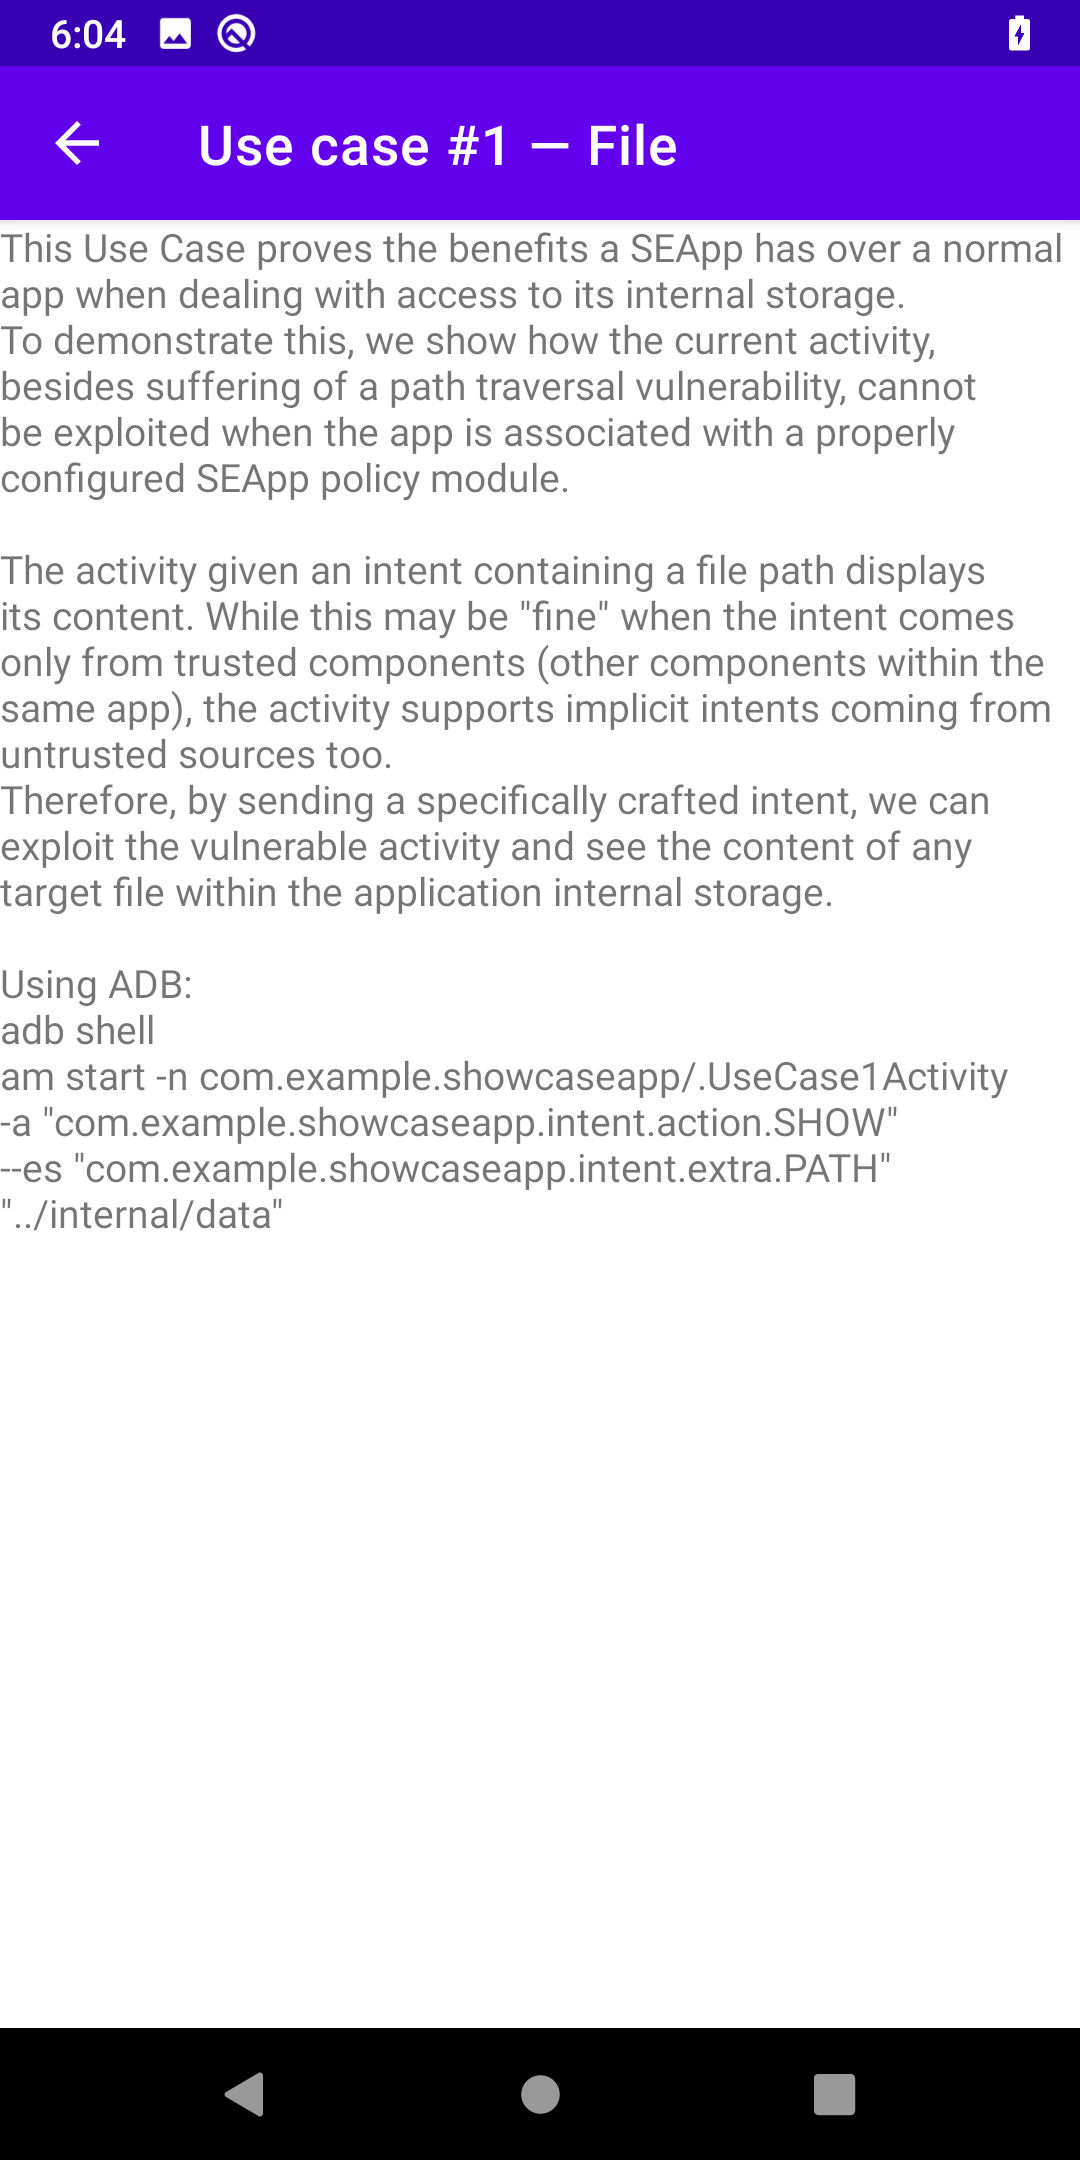
\includegraphics[width=0.28\textwidth]{chapters/seapp/figs/ae/UseCase1Activity.png}}
  \hfill
  \subfloat{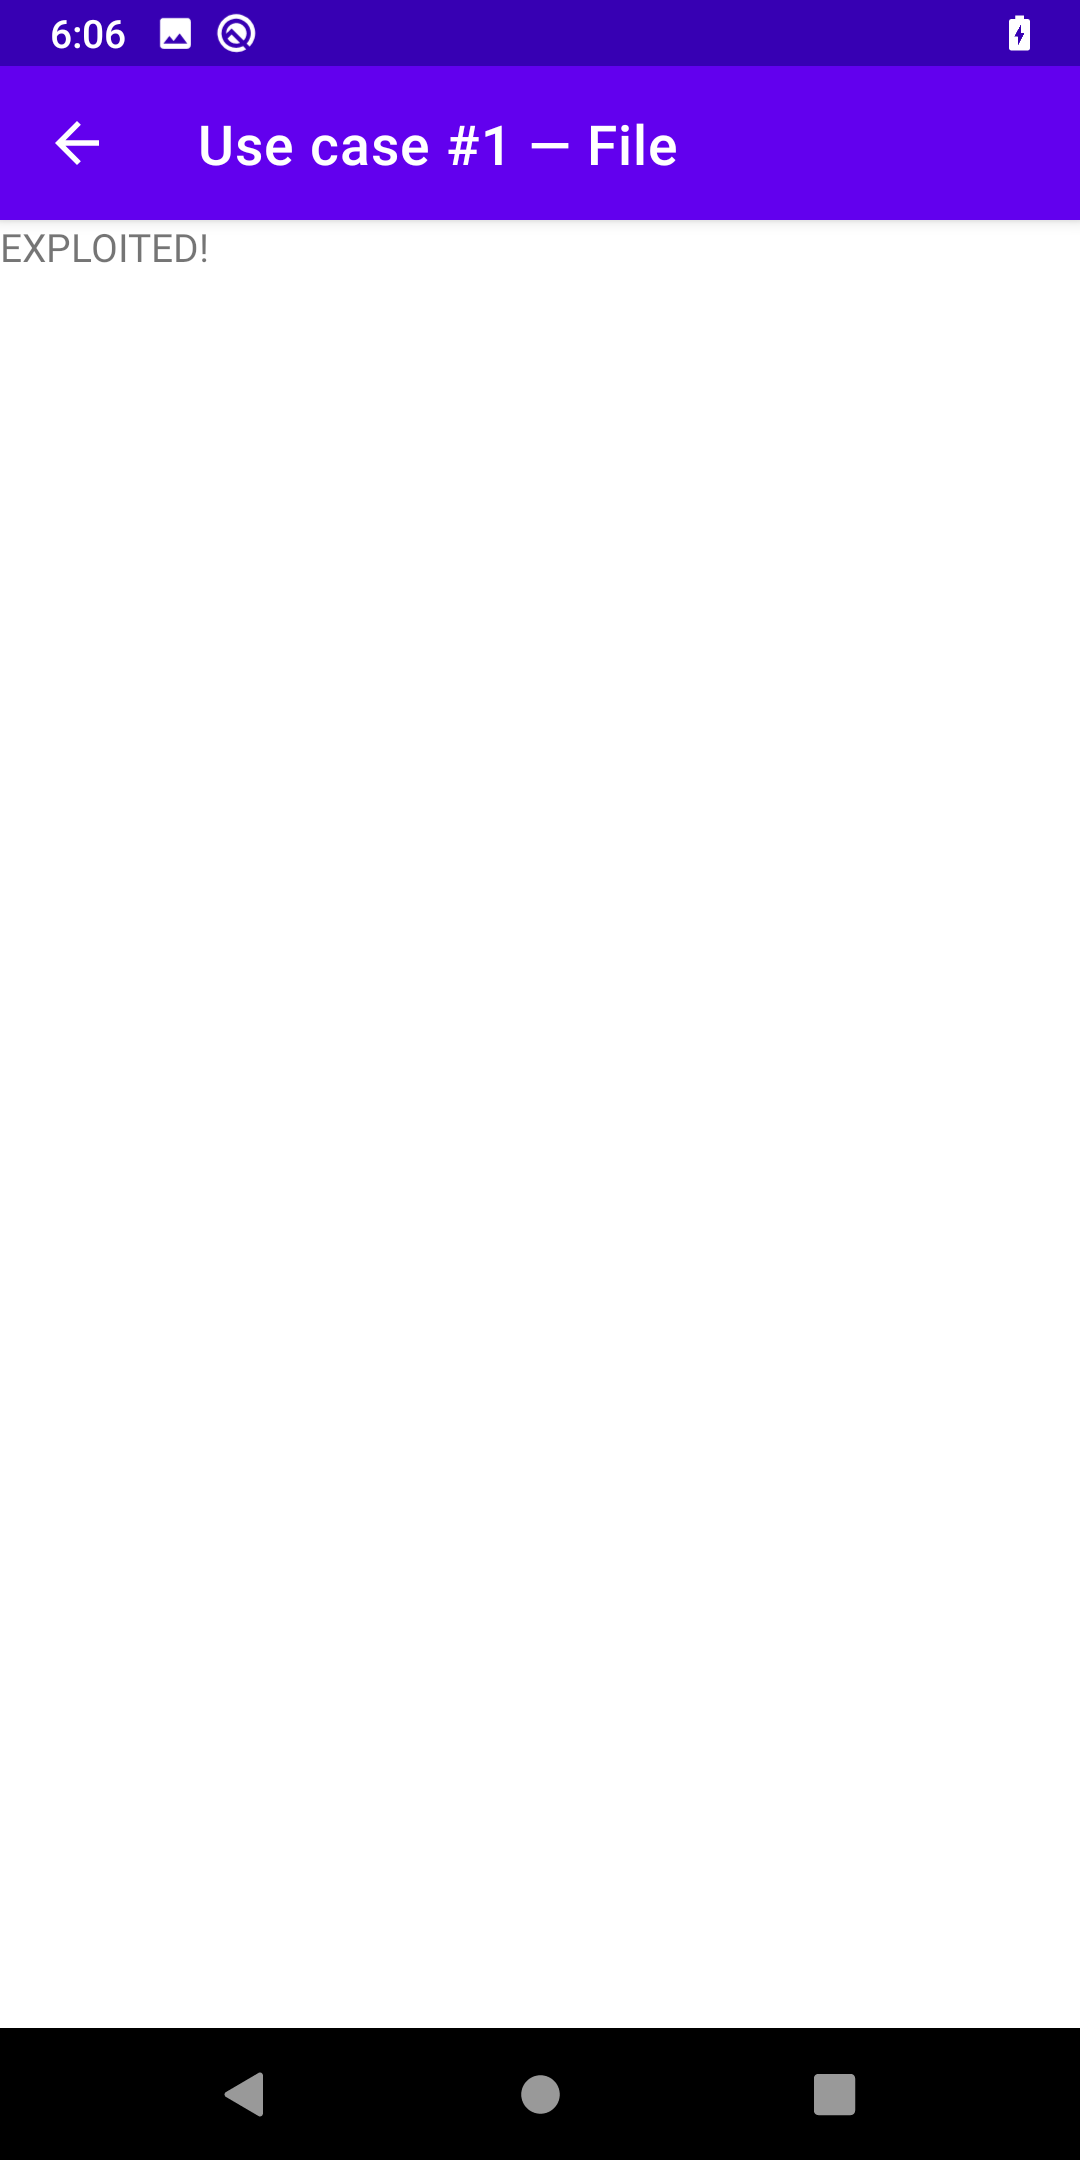
\includegraphics[width=0.28\textwidth]{chapters/seapp/figs/ae/UsaCase1ActivityExploited.png}}
  \hfill
  \subfloat{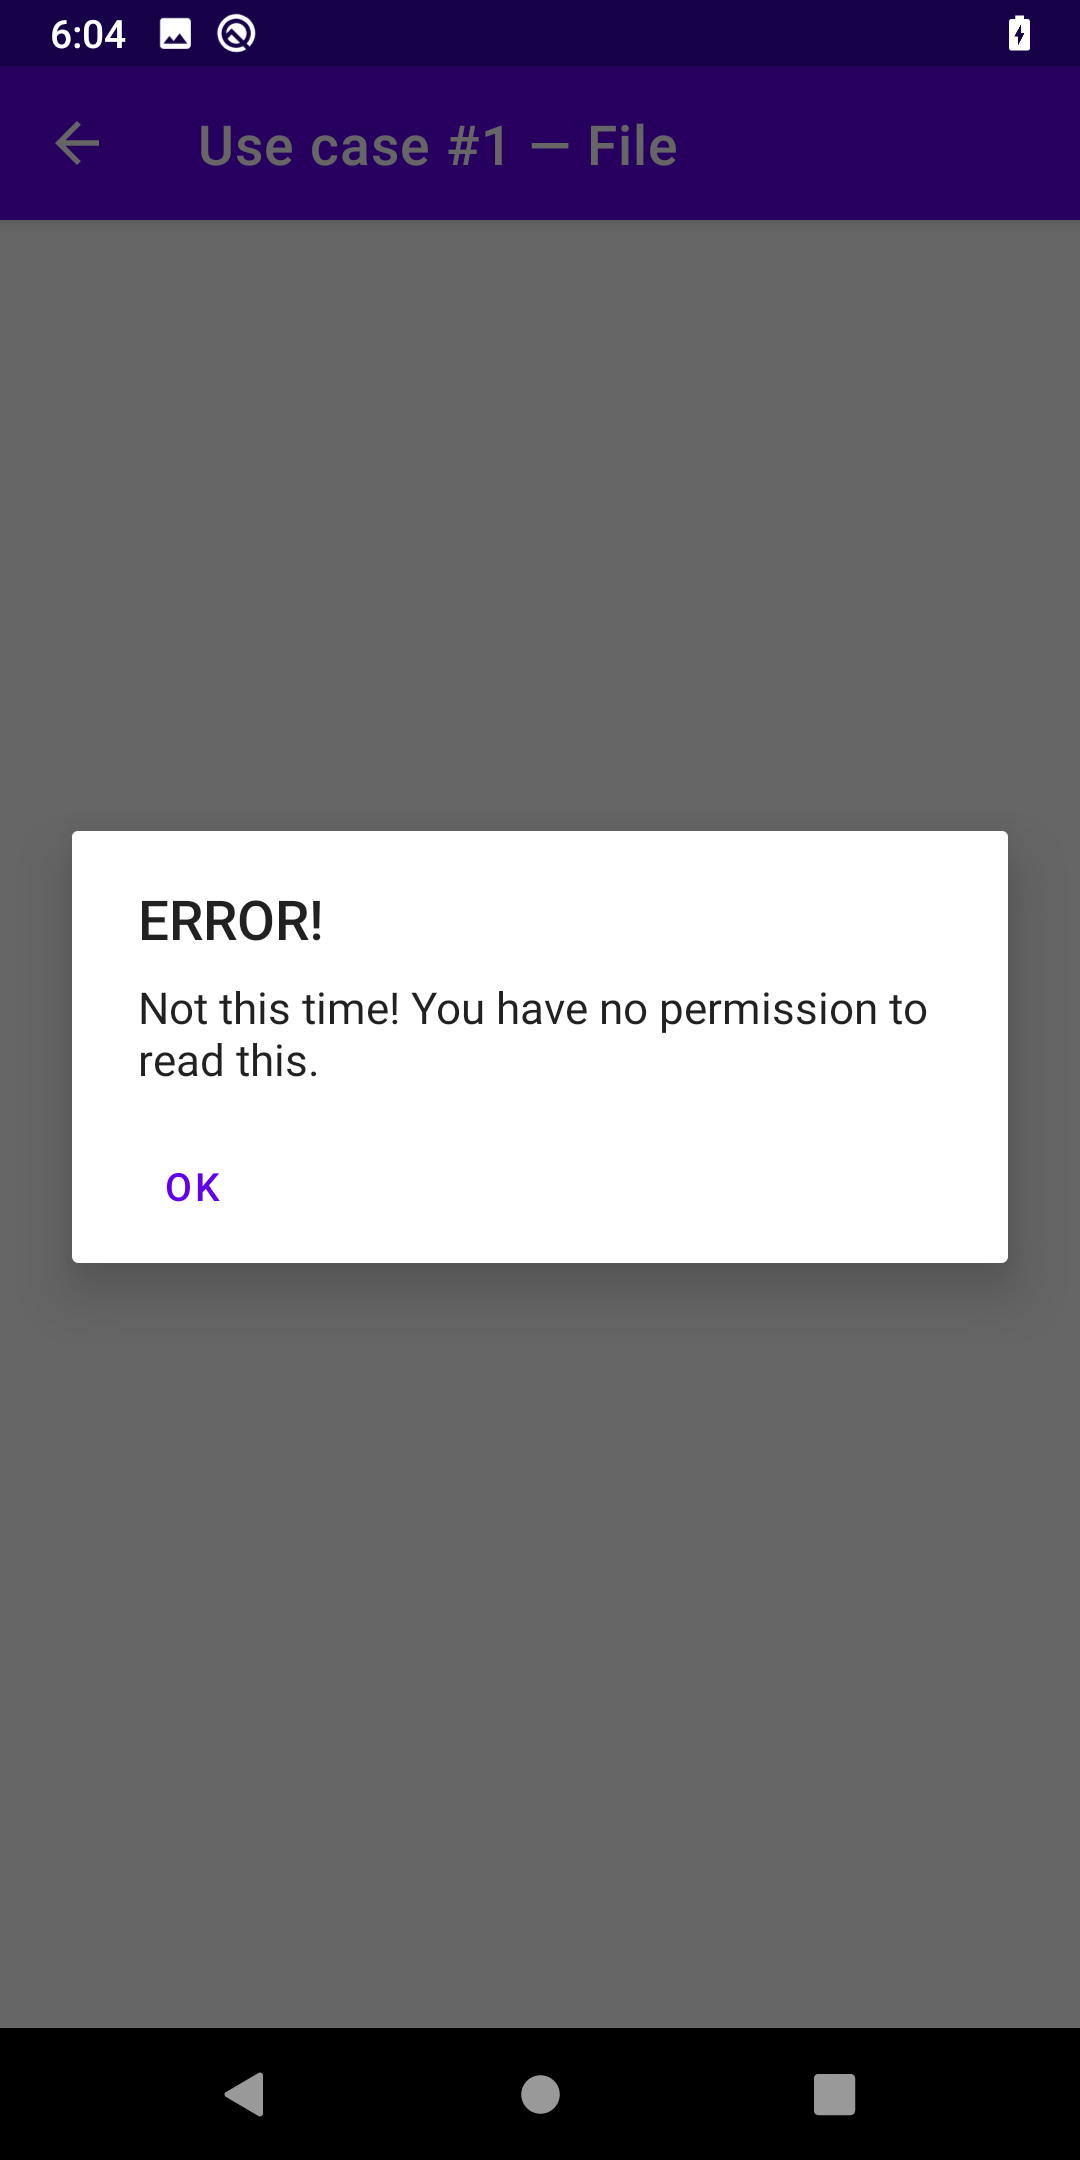
\includegraphics[width=0.28\textwidth]{chapters/seapp/figs/ae/UseCase1ActivityNotExploited.png}}
  \caption{\label{fig:seapp_uc1_views}\bf Use case 1 views}
\end{figure}

\begin{figure}[h!]
  \centering
  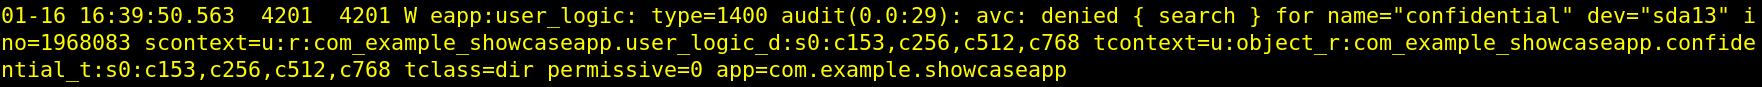
\includegraphics[width=\textwidth]{chapters/seapp/figs/ae/UseCase1Logcat.png}
  \caption{\label{fig:seapp_uc1_logcat}\bf Use case 1 logcat}  
\end{figure}

\newpage
      

%%% Local Variables: 
%%% mode: latex
%%% TeX-master: "../../../../main.tex"
%%% reftex-default-bibliography: "../../../../bib/biblio.bib"
%%% End:
